\documentclass[11pt]{article}
\usepackage[margin=1in]{geometry}
\usepackage{booktabs}
\usepackage{array}
\usepackage{longtable}
\usepackage{graphicx}
\usepackage[hidelinks]{hyperref}
\usepackage{amsmath}
\renewcommand{\thetable}{S\arabic{table}}
\renewcommand{\thefigure}{S\arabic{figure}}
\setlength{\parindent}{0pt}
\setlength{\parskip}{0.6em}

\title{Supplementary Information\\
\large Protocol-Dependent Performance in Rotating Machinery Fault Diagnosis:\\Evidence from Sealed Compound Generalization}
\author{Zixuan Liu}
\date{}

\begin{document}
\maketitle

\section*{S1. Evidence tiers and access states}

The Sealed Compound Generalization Protocol (SCGP) is a prospective evaluation contract. The empirical evidence in the manuscript is labeled according to the strongest retained access history that it supports. The HANOI HUST compound track is a historical held-out confirmation under a documented local freeze. The three-code Paderborn pilot is a one-shot external scoring run, and the disjoint 12-code extension was frozen locally before its numeric archives were accessed.

\begin{table}[h]
\centering
\small
\caption{Access-state contract used in the manuscript.}
\begin{tabular}{p{0.12\textwidth}p{0.28\textwidth}p{0.22\textwidth}p{0.27\textwidth}}
\toprule
State & Partition and access & Evaluation unit & Role \\
\midrule
P0 & Window-random; labels open & Window & Descriptive leakage diagnostic; excluded from primary inference \\
P1 & Record-grouped; labels open & Record or bearing-aggregated endpoint & Loose primary reference; records from one bearing may cross partitions \\
P2 & Bearing-grouped; labels open & Physical bearing & Leakage-controlled source comparison \\
P3 & Nested bearing-grouped selection & Physical bearing & Selection-adjusted source estimate \\
P4 & Confirmation access sealed by protocol & Physical bearing or declared external unit & Prospective confirmation state \\
\bottomrule
\end{tabular}
\end{table}

The source-only information budget, denoted I0, permits HANOI source records and registered source metadata during model fitting and selection. It excludes numeric values and labels from the HANOI compound partition and from external boundary sets.

\section*{S2. Primary G2 partition--aggregation audit}

The first two rows of Table~\ref{tab:s-g2} form the fixed-reference $2\times2$ comparison: partitioning varies between record-grouped and bearing-grouped, and the endpoint varies between record level and bearing aggregated. The third row adds nested selection within bearing-grouped outer folds.

\begin{table}[h]
\centering
\small
\caption{Primary G2 repeated-split means across 100 registered splits.}
\label{tab:s-g2}
\begin{tabular}{lrrrr}
\toprule
Protocol cell & Record AUROC & Record exact & Bearing AUROC & Bearing exact \\
\midrule
Record-grouped, fixed & 0.951 & 0.776 & 0.959 & 0.791 \\
Bearing-grouped, fixed & 0.828 & 0.510 & 0.860 & 0.490 \\
Bearing-grouped, nested & 0.777 & 0.420 & 0.803 & 0.406 \\
\bottomrule
\end{tabular}
\end{table}

Across the 100 nested outer folds, logistic--envelope configurations were selected 54 times, extra-trees--envelope configurations 29 times, and RBF-SVM--envelope configurations 17 times. The split-level results are correlated resamples of the same 19 physical bearings and are not treated as independent experiments.

\section*{S3. Secondary G3 model-family audit}

All methods in Table~\ref{tab:s-g3} use the same 100 bearing-grouped outer splits, the I0 source-only information budget, and physical-bearing aggregation. This secondary audit leaves the primary model choice unchanged.

\begin{table}[h]
\centering
\small
\caption{Source-only model-family comparison.}
\label{tab:s-g3}
\begin{tabular}{lrrrrr}
\toprule
Method & AUROC & AUPR & Balanced accuracy & Macro-F1 & Exact set \\
\midrule
Fixed logistic reference & 0.860 & 0.843 & 0.712 & 0.675 & 0.490 \\
Random forest & 0.785 & 0.750 & 0.666 & 0.628 & 0.458 \\
GroupDRO-style logistic & 0.845 & 0.825 & 0.721 & 0.680 & 0.482 \\
MiniROCKET & 0.751 & 0.708 & 0.682 & 0.628 & 0.556 \\
WDCNN-style & 0.630 & 0.608 & 0.530 & 0.386 & 0.116 \\
ResNet1D & 0.609 & 0.607 & 0.521 & 0.373 & 0.120 \\
InceptionTime-style & 0.569 & 0.565 & 0.516 & 0.370 & 0.120 \\
\bottomrule
\end{tabular}
\end{table}

For the paired GroupDRO comparison, the mean split-level AUROC difference (GroupDRO minus fixed logistic) was $-0.015$. A deterministic 200,000-draw sign-permutation calculation gave a two-sided $p$ value of 0.0063. Because all splits reuse the same 19 bearings, this value is a conditional resampling summary rather than evidence from 100 independent experiments.

\section*{S4. Legacy NOACE comparator statistics}

The legacy audit predates the matched G2/G3 analysis and uses a different candidate pool and endpoint. Its results are retained for provenance under their original access state.

\begin{table}[h]
\centering
\small
\caption{Legacy 19-bearing source comparison.}
\label{tab:s-noace}
\begin{tabular}{lrrrrr}
\toprule
Setting & AUROC & Balanced accuracy & Exact set & Brier & Hamming \\
\midrule
SCGP source reference & 0.814 & 0.743 & 0.544 & 0.161 & 0.199 \\
NOACE-classical & 0.809 & 0.742 & 0.579 & 0.216 & 0.211 \\
\bottomrule
\end{tabular}

\vspace{0.6em}
\begin{tabular}{lrrrr}
\toprule
Comparator & Exact set & Difference (pp) & 95\% CI & Holm-adjusted $p$ \\
\midrule
NOACE-classical & 0.579 & $-3.51$ & [$-28.1$, 21.1] & 1.000 \\
NOACE-physics & 0.579 & $-3.51$ & [$-28.1$, 21.1] & 1.000 \\
NOACE-deep & 0.544 & 0.00 & [$-17.5$, 15.8] & 1.000 \\
\bottomrule
\end{tabular}
\end{table}

Here, the difference is the source-reference minus comparator difference in bearing-level exact-set accuracy. Confidence intervals use 10,000 bearing-cluster bootstrap resamples. The inferential support consists of 19 physical bearings.

\begin{figure}[htbp]
\centering
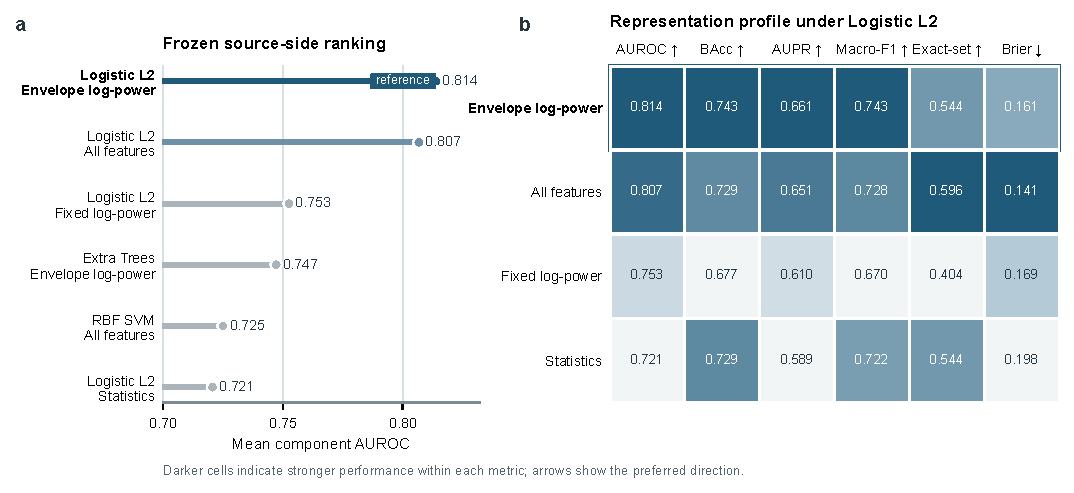
\includegraphics[width=\textwidth]{figures/figure2_source_champion.pdf}
\caption{Legacy frozen source reference and representation profile. (a) Six model--representation pairs ranked by mean component AUROC on 19 source bearings. (b) Four representations compared with \texttt{logistic\_l2}; darker cells denote better performance after reversing the Brier-score direction. \texttt{envelope\_log\_power} leads component discrimination, whereas \texttt{all} has higher exact-set accuracy and a lower Brier score. Values retain the endpoint and access state of the legacy audit.}
\label{fig:s-source-champion}
\end{figure}

\begin{figure}[htbp]
\centering
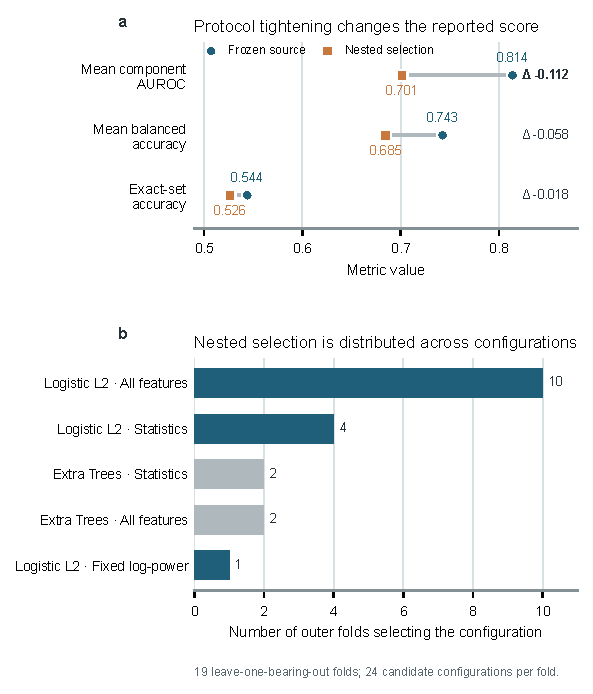
\includegraphics[width=0.72\textwidth]{figures/figure4_protocol_sensitivity.pdf}
\caption{Legacy protocol tightening and selection stability. (a) Frozen source and nested physical-unit point estimates for mean component AUROC, balanced accuracy, and exact-set accuracy on 19 source bearings. Lines show state-specific changes; distinct metrics are not averaged. (b) Family--representation selections across 19 outer folds after pooling hyperparameters. Each fold screens 24 configurations. Counts are selection frequencies, not uncertainty estimates, and candidate pools differ across access states.}
\label{fig:s-protocol-sensitivity}
\end{figure}

\section*{S5. HANOI HUST held-out compound boundary}

The held-out HANOI HUST track contains 14 compound bearings. The fixed logistic--envelope reference achieved mean component AUROC 0.811 and exact-set accuracy 2/14. NOACE-classical and the MLP comparator produced exact-set accuracy 0/14. Resampling 14 identical zero outcomes gives a degenerate empirical bootstrap interval of 0--0. A two-sided Clopper--Pearson sensitivity interval for 0/14 is 0--0.232, which better communicates population uncertainty beyond the observed boundary.

This track is described as a historical held-out confirmation under a documented local freeze. It is not described as a publicly time-stamped prospective lockbox.

\section*{S6. Supplementary heterogeneous boundary checks}

The Mendeley Pump and Zenodo 14388093 analyses use different tasks, algorithms, and evaluation units from HANOI HUST. They are retained as supplementary checks and are not treated as replications of the HANOI classifier.

\begin{table}[h]
\centering
\small
\caption{Supplementary heterogeneous boundary results.}
\begin{tabular}{p{0.19\textwidth}p{0.25\textwidth}p{0.43\textwidth}}
\toprule
Resource & Evaluation unit & Recorded result and interpretation \\
\midrule
Mendeley Pump & 24 state workbooks & Source anchors were recovered for 9/9 states. Unseen exact recovery was 3/15 and generalized exact recovery was 12/24. Each workbook contributes one state-level external unit. \\
Zenodo 14388093 & 320 records from one rig at four speeds & The source-safe reference reached component balanced accuracy 1.000 and exact-set accuracy 1.000. Generalized values were 0.875 and 0.750. The track provides a single-rig external check. \\
\bottomrule
\end{tabular}
\end{table}

\section*{S7. Paderborn three-code pilot registry}

The three-code pilot contains K001 (healthy), KA01 (outer-race damage), and KI01 (inner-race damage), with 80 records per code and 240 records in total. The source-trained logistic--envelope model, fold-fitted scaling rule, and threshold 0.5 were fixed before external scoring. No Paderborn record or label was used for model selection or threshold tuning.

The three-code registry is independent of an earlier 15-code confirmatory registry. That earlier registry retained \texttt{numeric\_access\_authorized: false}, contained different bearing codes, and was never scored as that protocol. The pilot registry, archive hashes, scoring script, feature cache, result JSON, and unit rows are included in Supplementary Data~S1.

At bearing-code level, the frozen reference recovered the healthy code but missed both damaged codes. Inner- and outer-race AUROC were 0.000, and exact-set accuracy was 1/3. This three-code result provides initial negative cross-rig evidence at the bearing-code endpoint.

\section*{S8. Disjoint 12-code Paderborn extension}

To increase independent-unit support, a new registry was frozen before numeric access. It selected four healthy codes (K002--K005), four outer-race codes (KA04, KA15, KA16, and KA22), and four inner-race codes (KI04, KI14, KI16, and KI18). All 12 codes are disjoint from K001, KA01, and KI01. The HANOI-only scaler, logistic--envelope model, $C=10$, threshold 0.5, record-to-code averaging rule, and uncertainty procedure were fixed before the official archives were downloaded. Paderborn labels were not used for model fitting, representation choice, or threshold tuning.

The 12 official RAR files matched their HTTP content lengths and yielded 80 MAT records each. Archive hashes, the registry hash, execution-script hash, derived feature-cache hash, and 960-record target mapping were retained. An independent audit rebuilt all code probabilities and headline metrics from the frozen source and external feature caches.

Inner-race AUROC was 0.344 (stratified bearing-code bootstrap 95\% CI, 0--0.688), and outer-race AUROC was 0.719 (0.250--1.000). Exact-set accuracy was 3/12, or 0.250 (95\% Clopper--Pearson CI, 0.055--0.572). Exact recovery by state was 2/4 (healthy), 0/4 (outer race), and 1/4 (inner race).

\begin{table}[htbp]
\centering
\small
\caption{Bearing-code outcomes for the pre-access-frozen Paderborn extension. Probabilities are ordered as inner race, outer race, and ball; targets and predictions use the same order.}
\label{tab:s-paderborn-extension}
\begin{tabular}{lccccc}
\toprule
Code & Target & $p_{\mathrm{inner}}$ & $p_{\mathrm{outer}}$ & $p_{\mathrm{ball}}$ & \shortstack{Prediction /\\exact} \\
\midrule
K002 & 000 & 0.284 & 0.005 & 0.000 & 000 / yes \\
K003 & 000 & 0.245 & 0.017 & 0.000 & 000 / yes \\
K004 & 000 & 0.728 & 0.004 & 0.000 & 100 / no \\
K005 & 000 & 0.628 & 0.004 & 0.000 & 100 / no \\
KA04 & 010 & 0.515 & 0.242 & 0.013 & 100 / no \\
KA15 & 010 & 0.400 & 0.029 & 0.000 & 000 / no \\
KA16 & 010 & 0.348 & 0.412 & 0.000 & 000 / no \\
KA22 & 010 & 0.528 & 0.001 & 0.000 & 100 / no \\
KI04 & 100 & 0.347 & 0.026 & 0.012 & 000 / no \\
KI14 & 100 & 0.587 & 0.021 & 0.000 & 100 / yes \\
KI16 & 100 & 0.287 & 0.016 & 0.002 & 000 / no \\
KI18 & 100 & 0.268 & 0.059 & 0.000 & 000 / no \\
\bottomrule
\end{tabular}
\end{table}

This extension increases the independent external support to four codes per state. Its one-rig design and absence of a Paderborn ball-fault state define the scope of the result, and its access record remains distinct from the pilot.

\section*{S9. Reproduction entry points}

Raw HANOI HUST and Paderborn waveform archives are not redistributed. Supplementary Data~S1 contains derived caches, predictions, manifests, audit records, and source code sufficient to inspect and reconstruct the reported tables from the retained derived data.

\small
\begin{longtable}{p{0.37\textwidth}p{0.55\textwidth}}
\toprule
Purpose & Entry point \\
\midrule
\endhead
Primary G2 execution & \texttt{src/run\_hanoi\_hust\_g2\_protocol.py} \\
Primary G2 audit & \texttt{src/audit\_hanoi\_hust\_g2\_main\_table.py} \\
Factorial endpoint audit & \texttt{src/audit\_hanoi\_hust\_factorial\_endpoints.py} \\
G3 model-family runs & \texttt{src/run\_hanoi\_hust\_g3\_*.py} \\
Legacy NOACE ablation & \texttt{src/run\_hanoi\_hust\_noace\_ablation.py} \\
Paderborn boundary run & \path{src/run_hanoi_hust_paderborn_external_lockbox.py} \\
Paderborn 12-code extension & \path{src/run_hanoi_hust_paderborn_twelve_code_extension.py} \\
Paderborn extension audit & \path{src/audit_paderborn_twelve_code_extension.py} \\
Physical-unit manifests & \texttt{results/g2/split\_manifests/} \\
Feature caches & \texttt{artifacts/hanoi\_hust/} \\
\bottomrule
\end{longtable}

\end{document}
